\documentclass[11pt,a4paper]{article}
\usepackage[margin=25mm]{geometry}
\usepackage{fontspec,unicode-math,amsmath,booktabs,graphicx,hyperref}
\setmainfont{STIXGeneral}\setmathfont{STIX Two Math}
\setlength{\parindent}{0pt}\setlength{\parskip}{6pt}
\title{Supported kernels, translation lattices\\and finite marked quotients}
\author{Comparison of ten complete originals}\date{}
\begin{document}\maketitle
The complete originals contain 319,016 characters. The complete common theory and applications contain 263,470 characters. Charging the common theory once within this topic gives
\[
R=\frac{\sum_{i=1}^{10}c(S_i)}{c(U)+\sum_{i=1}^{10}c(A_i)}
=\frac{319016}{108271+155199}
=1.210825.
\]
Here $c$ counts nonspace characters in the accepted, selected and calibrated PDF extraction after NFC normalization. The convention is unchanged from the previous comparison. It measures these written proofs and their exposition; it does not estimate minimum proof length or historical originality.

All 152 source pages, all 41 common pages and all 63 application pages are included. The common theory comprises the unchanged 23-page paper (66,140 characters), the complete 14-page supplement (33,986) and the four-page structural argument (8,145). Each is paid in full. Titles, abstracts, proofs, tables, references, addresses and extracted figure labels remain.

\textbf{Individual factors after acquiring the common theory.}
The factors below are $c(S_i)/c(A_i)$. Their prerequisite is the entire common theory, all 99 required program and data contents, and the retained external mathematical premises. Every application is complete; no sibling application is a free premise.
\begin{center}\begin{tabular}{llrrr}\toprule
Original & App & Source & Application & Factor\\\midrule
L032 & A1 & 16,558 & 8,228 & 2.012397\\
L034 & A2 & 21,433 & 5,801 & 3.694708\\
F016 & A3 & 43,983 & 15,436 & 2.849378\\
F013 & A4 & 25,562 & 6,241 & 4.095818\\
L035 & A5 & 51,019 & 14,514 & 3.515158\\
N009 & A6 & 36,824 & 28,130 & 1.309065\\
L128 & A7 & 18,424 & 8,825 & 2.087705\\
L012 & A8 & 32,767 & 23,401 & 1.400239\\
L121 & A9 & 27,367 & 2,227 & 12.288729\\
L003 & A10 & 45,079 & 42,396 & 1.063284\\
\bottomrule\end{tabular}\end{center}
The first eight individual factors are unchanged. L121 now has a one-page application: its four substantial proof bodies have moved into the paid common supplement. L003 includes its entire 17-page application, comprising the seven-page main text and companions of four, four and two pages.
\newpage
\begin{center}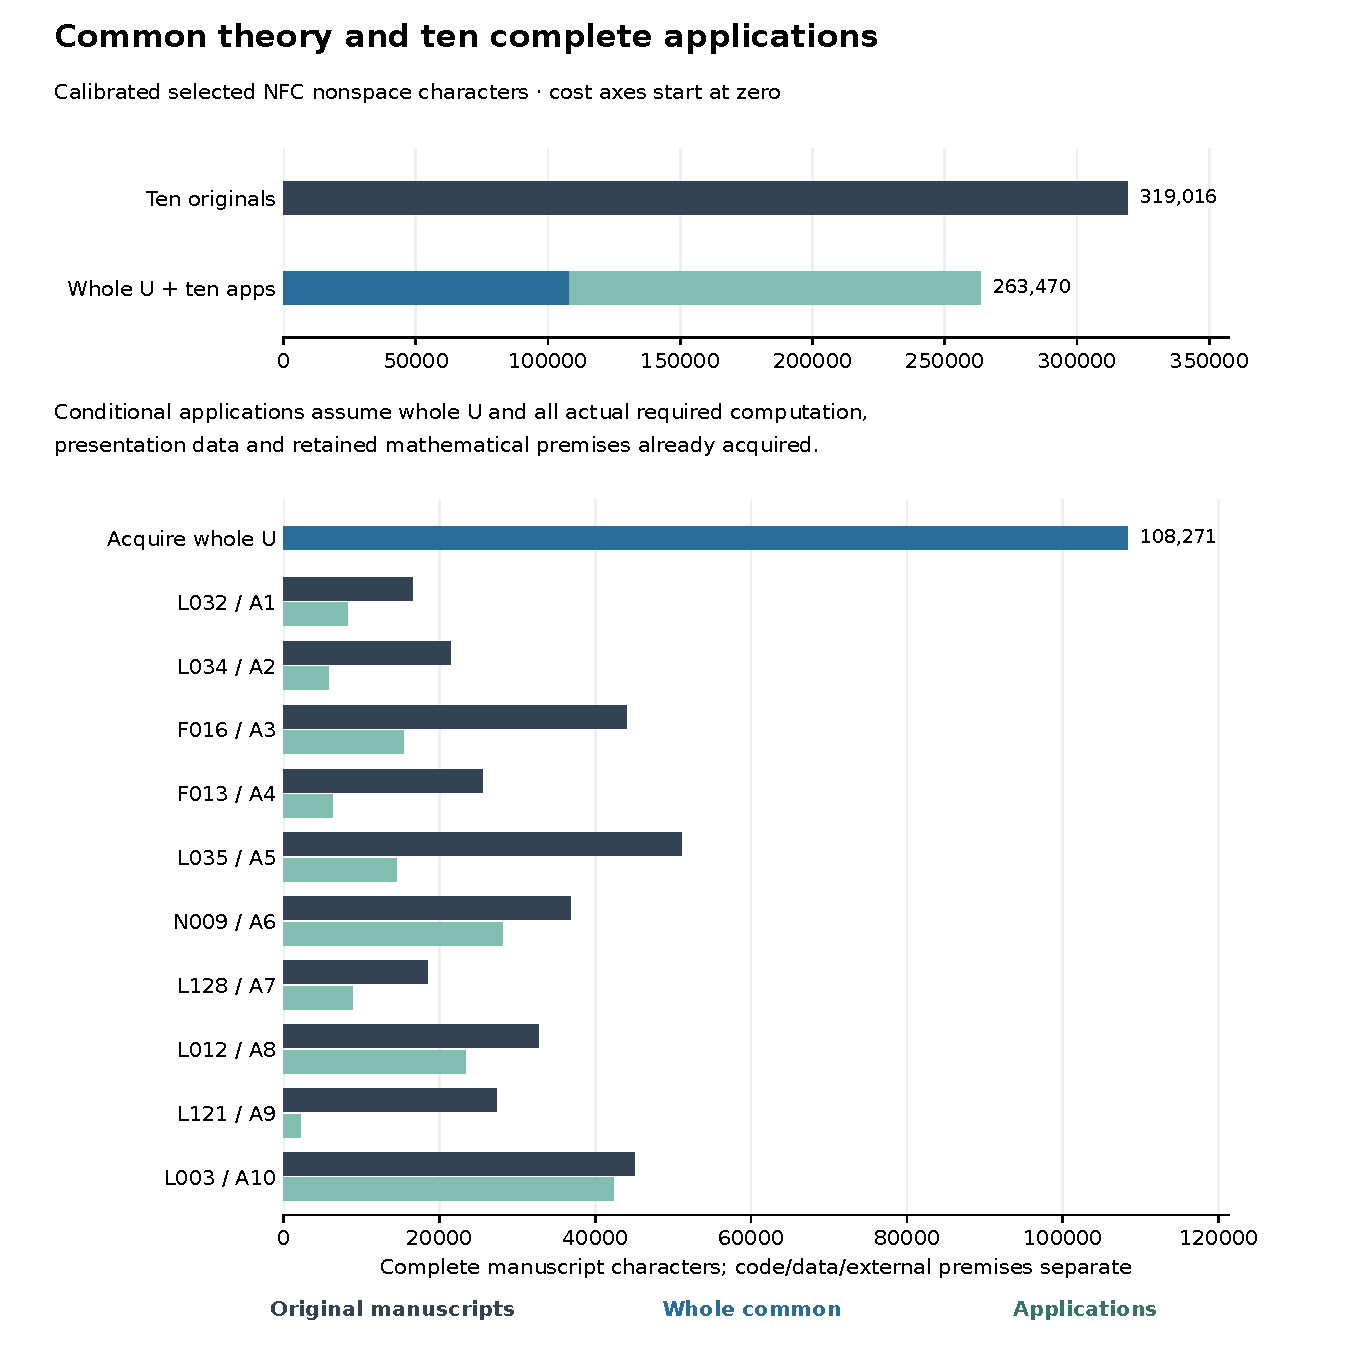
\includegraphics[width=\textwidth]{costs.pdf}\end{center}
Both charts use complete manuscript costs and axes beginning at zero. The upper replacement bar includes all three common components and all ten applications. The lower chart shows common acquisition followed by each source/application pair. These 35 bars represent text length, not theorem counts or ratios.

The larger common theory makes L121 a short corollary, but it has an acquisition cost. The complete factor decreases from 1.354347 for nine originals to 1.210825 for ten. The source side gains 45,079 characters; common material gains 42,131; replacing the old L121 application saves 23,322; and L003 adds 42,396 application characters. The net replacement increase is 61,205. Both editions remain available for comparison.
\newpage
\begin{center}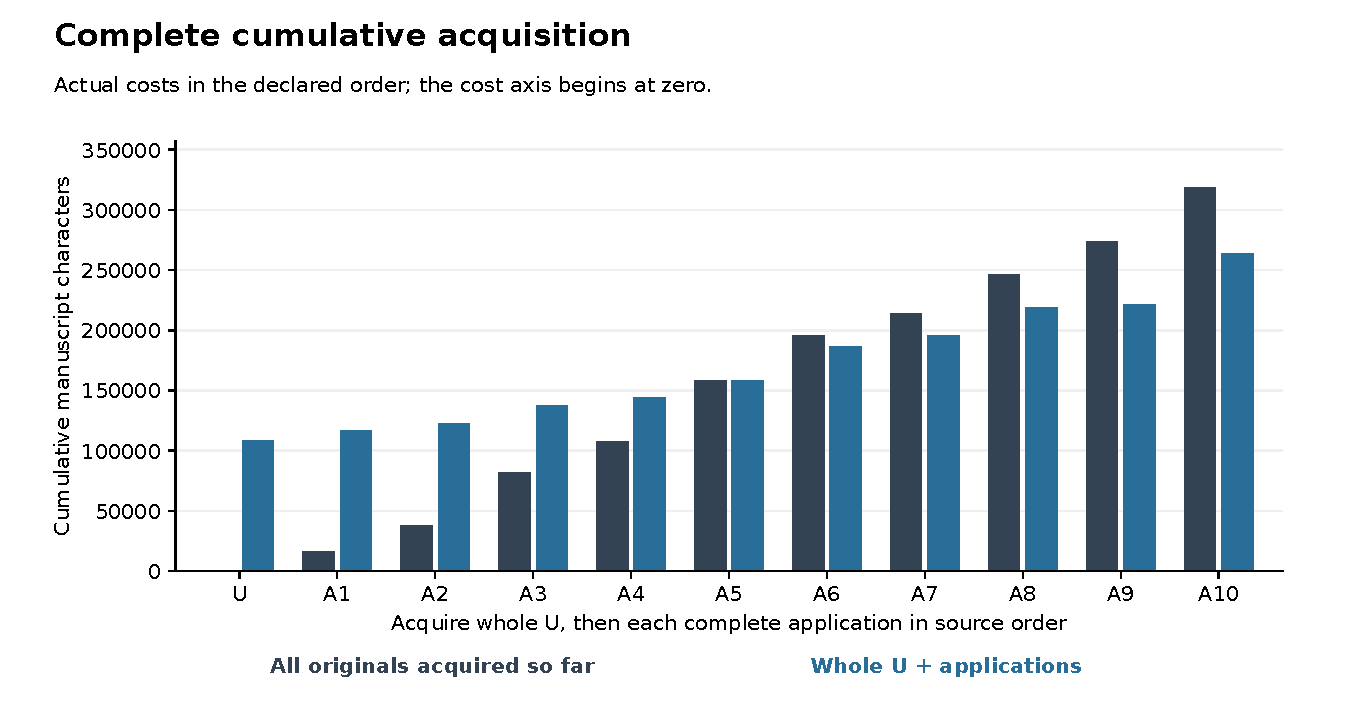
\includegraphics[width=\textwidth]{cumulative.pdf}\end{center}
Stage zero acquires the entire common theory. Each subsequent stage adds one complete original and its complete application, in the inherited documentary order followed by L003. The eleven cumulative stages use actual costs. No optimal ordering or general sawtooth law is inferred from this one sequence.

\textbf{Separate complete file inventory.}
\begin{center}\small\begin{tabular}{lrrr}\toprule
Whole contents & Count & NFC nonspace & Literal bytes\\\midrule
Required programs & 28 & 102,679 & 114,947\\
Required data & 71 & 856,967 & 992,789\\
Operational files & 17 & 83,928 & 92,190\\
Optional validation & 5 & 8,617 & 10,015\\
Partial formal files & 16 & 70,785 & 100,644\\
Output receipts & 66 & 5,229,020 & 5,579,535\\
\bottomrule\end{tabular}\end{center}
All 253 file occurrences resolve to 203 distinct complete contents. Their accounting classes are disjoint; the original overlapping roles and every file route remain recorded. Data consumed by a proof stays required even when it was produced by an earlier calculation. The complete 28 programs and 71 data contents remain prerequisites.

Executable code is excluded from both sides of the written comparison. Mathematical algorithms described in prose remain. Historical software costs are unknown, so no software-inclusive ratio is reported. The three earlier printed program appendices cover only the old eleven-file subset. Their 30 pages are separate historical representations, never an additional written-proof cost or a complete representation of the enlarged software collection. Partial formal files do not establish complete formalization.
\newpage
\textbf{Sensitivity of the complete written factor.}
\begin{center}\small\begin{tabular}{lrrr}\toprule
Unit & Raw complete & Raw selected & Calibrated\\\midrule
NFC: Whitespace tokens & 1.399961 & 1.387281 & 1.387249\\
NFC: Alphanumeric units & 1.455399 & 1.440722 & 1.442273\\
NFC: Nonspace characters & 1.225689 & 1.210807 & 1.210825\\
NFC: Collapsed-space characters & 1.256597 & 1.242070 & 1.242079\\
NFC: Collapsed UTF-8 bytes & 1.223269 & 1.209790 & 1.209547\\
NFKC: Whitespace tokens & 1.402153 & 1.389477 & 1.389446\\
NFKC: Alphanumeric units & 1.455399 & 1.440722 & 1.442273\\
NFKC: Nonspace characters & 1.227194 & 1.212319 & 1.212337\\
NFKC: Collapsed-space characters & 1.258214 & 1.243694 & 1.243703\\
NFKC: Collapsed UTF-8 bytes & 1.302717 & 1.288402 & 1.286938\\
\bottomrule\end{tabular}\end{center}
All thirty coordinates and 330 exact fractions are supplied in JSON and CSV. Each fraction retains the unreduced manuscript costs, reduced numerator and denominator, and twelve-place decimal. The previous eight conditional records are unchanged in all thirty coordinates. The 870 PDF cells and 2,030 raw-content cells come from the accepted input audit; this calculation performs no new extraction.

Raw complete text includes running headers and page numbers. Selection removes only their exact audited occurrences. Calibration repairs actual mathematical glyph aliases using the embedded font, encoding and text event. It preserves both visible braces that decoded as TAB, and keeps mapsto components separate. Ordinary ligatures and printed hyphens are not rewritten. NFC and NFKC remain separate sensitivities.

L003 contains 423 occurrences of drawing-font aliases, retained literally and identified separately. They are representation tokens, not a transcription of mathematical or linguistic content. Extracted labels remain, while full graphical structure and unextracted image labels have unknown cost. The scalar therefore measures extraction representation length; it does not price geometric information. Installed libraries, retained external classifications and proof libraries, historical software and complete formalization costs also remain unknown.

\textbf{Scope and attribution.} The previously accepted corrected recovery is the mathematical basis of this comparison. Its order corrections, nonsplitting result, local-period qualifications and precise universal-presentation hypotheses remain in force. Source experiments and conjectures receive no new proof credit from this numerical packet. Ten originals remain ten originals regardless of the number of individual claims or finite checks.

Root authored this arithmetic after separately reviewing the input audit. Earlier fraction, CSV and plotting mechanics are adapted from the accepted L121 comparison; the vector-geometry checker is reused unchanged. The input author and numerical reviewer are identified separately. A fresh numerical review is required before public admission. No mathematical enumeration or Lean compilation is repeated here.
\end{document}
